%! TeX program = lualatex
%tags! intro first class databases
\documentclass[letterpaper]{article}
\usepackage[margin=1in]{geometry}
\usepackage{amsmath}
\usepackage{amssymb}
\usepackage[no-math]{fontspec}
\usepackage[bg,fg]{gruvboxpalette}
\usepackage{graphicx}
\graphicspath{{.}}
\usepackage{hyperref}
\usepackage{newtxsf}
\usepackage[explicit]{titlesec}
\usepackage{tikz}
\usetikzlibrary{calc}
\usetikzlibrary{positioning}
\usetikzlibrary{arrows.meta}
\usepackage[most]{tcolorbox}
\usepackage{tabularray}
\DefTblrTemplate{firsthead, middlehead,lasthead}{default}{}
\DefTblrTemplate{capcont}{default}{}
\DefTblrTemplate{contfoot-text}{normal}{} \SetTblrTemplate{contfoot-text}{normal} \DefTblrTemplate{conthead-text}{normal}{} \SetTblrTemplate{conthead-text}{normal}
\UseTblrLibrary{counter}
\hypersetup{
  colorlinks  = true,
  urlcolor    = Blue,
  linkcolor   = Blue,
  citecolor   = Blue
}
\usepackage[most]{tcolorbox}

\setmainfont{NotoSans-Regular}[
Path           = /home/snouflake/.fonts/ ,
Extension      = .ttf ,
BoldFont       = NotoSans-Bold ,
ItalicFont     = NotoSans-Italic ,
BoldItalicFont = NotoSans-BoldItalic,
] 

\newtcolorbox{defbox}[2][]{%
  colback=blue!30!background,
  coltitle=blue!15!black,
  coltext=font,
  title filled=false,
	enhanced,
  detach title,
  tile,
  before upper={\tcbtitle\medskip\\},
  borderline west={2mm}{0pt}{blue},
  % attach boxed title to top center={yshift=-2mm},
  leftrule=2mm,
  toprule=0mm,
  bottomrule=0mm,
  rightrule=0mm,
  arc=0mm,
	title={Definición:~#2},
	#1
}

\setlength\parindent{0pt}

\usepackage{mathastext}

\def \T{Bases de datos}
\def \S{Introducción}

\begin{document}
\begin{tikzpicture}[inner sep=0pt,color=font]
  \node[anchor=west,align=left,text width=\linewidth-2pt] 
    (title) at (0,0.9) {\Huge\bfseries\T};
  \node[anchor=west,align=left] 
    (subtitle) at (0,-0.5) {\Large\bfseries\S};
\end{tikzpicture}
\vspace{16pt}

\section*{¿Cómo debe ser el almacenamiento de una base de datos?}
\vspace{-1cm}
\begin{longtblr}{
    colspec={@{}Q[h,4cm,cmd=\textbf] X[t]@{}},
    rowsep={7pt},
  }
  Registro 
  & {
    Debe ser rápido; un registro lento puede significar una pérdiad de usuarios.
  }
  \\
  Recuperación
  & Debe ser rápida y sencilla, a pesar de la cantidad de datos.
  \\
  Permanencia
  & El almacenamiento debe de ser confiable; garantizar que los datos no se pierdan.
  \\
  Localización
  & Toda la información debe poderse localizar de manera sencilla en cualquier momento.
\end{longtblr}

\section*{¿Qué es un sistema de bases de datos?}
\vspace{-1cm}
\begin{longtblr}{
    colspec={@{}Q[h,4cm,cmd=\textbf] X[t]@{}},
    rowsep={7pt},
  }
  Componentes 
  & \begin{minipage}{\linewidth}
    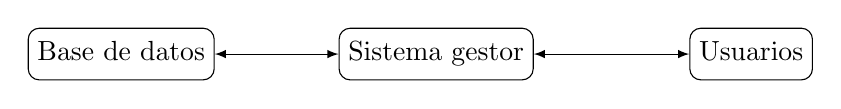
\begin{tikzpicture}
      \node[rounded corners,draw] (db) at (0,0) {\strut Base de datos};
      \node[rounded corners,draw] (dbms) at (4,0) {\strut Sistema gestor};
      \node[rounded corners,draw] (user) at (8,0) {\strut Usuarios};
      \draw[<->,>=latex] (db) to (dbms);
      \draw[<->,>=latex] (user) to (dbms);
    \end{tikzpicture}
  \end{minipage}
  \\
  Sistema jerárquicos
  & \begin{minipage}{\linewidth}
    \begin{itemize}
      \item Estructura de árbol 
      \item Incapaz de dvitar redundancia de información 
      \item Al borrar el nodo padre, se eliminan los hijos 
      \item Un nodo solo puede tener un nodo padre
    \end{itemize}
  \end{minipage}
  \\
  Sistema relacional
  & \begin{minipage}{\linewidth}
    \begin{itemize}
      \item Una colección organizada de información relacionada 
      \item Los datos se representan en tablas 
      \item Evida la redundancia de información 
      \item Facilita gestionar la información 
      \item Autodescriptiva: Contiene la descripción de su propia estructura 
      \item Integrada: Incluye las relaciones de las tablas que la conforman
    \end{itemize}

    {\bfseries Elementos}
    \begin{itemize}
      \item Base de datos: tabla y metadatos
      \item Tabla 
      \item Atributos: campos / columnas
      \item Registro: los datos contenidos en los atributos 
      \item Diccionario de [meta]datos: datos sobre la tabla- nombres de atributos, sus tipos de dato, su descripción
    \end{itemize}
  \end{minipage}
\end{longtblr}

\section*{Arquitectura}
\vspace{-1cm}
\begin{longtblr}{
    colspec={@{}Q[t,4cm,cmd=\textbf] X[t]@{}},
    rowsep={7pt},
  }
  Nivel externo, front end
  & Cómo el end user accede a los datos 
  \\
  Nivel conceptual
  & Estructura interna, diseñada por los programadores de la aplicación, se basa en las necedidades del usuario final
  \\
  Nivel interno
  & Instalación, configuración, seguridad, permisos, actualizaciónes, auditar accesos, resguardar la información
\end{longtblr}

\section*{Entorno}
Elementos y herramientas que interactuan para gestionar y usar la base de datos. Incluye a los componentes técnicos y a las personas involucradas.

% \vspace{-1cm}
\begin{longtblr}{
    colspec={@{}Q[t,4cm,cmd=\textbf] X[t]@{}},
    rowsep={7pt},
  }
  Procedimientos
  & Las políticas y reglas para el manejo de la base de datos
  \\
  Software
  & DB, DBMS, OS, seguridad, respaldo, monitoreo
  \\
  Hardware
  & Almacenamiento, servidores, memoria, redes
  \\
  Personas
\end{longtblr}

\end{document}

